\clearpage
\section{Implications for HL-LHC processes}
\label{sec:pheno}

The reduction of PDF uncertainties enabled by the neutrino DIS measurements
at the FPF presented in Sect.~\ref{sec:protonPDFs}
makes possible more precise theoretical predictions for key processes at the
HL-LHC.
%
Here we present an initial study of the phenomenological implications
of PDFs enhanced with LHC neutrino data.
%
We adopt the same settings as in the LHC phenomenology analysis presented
in the PDF4LHC21 combination paper~\cite{PDF4LHCWorkingGroup:2022cjn} and provide predictions
both for inclusive fiducial cross-sections and for differential distributions.
%
Specifically, we present results for 
single and double gauge boson production, inclusive top quark pair production,
and Higgs production in gluon
fusion and in association with a vector boson.
%
We evaluate these cross-sections using NLO matrix elements
which include  both in the
QCD and electroweak corrections using
{\sc\small mg5\_amc@nlo}~\cite{Frederix:2018nkq}
interfaced to {\sc\small PineAPPL}~\cite{Carrazza:2020gss}.
%
For all processes, realistic selection and acceptance cuts on the final state particles
have been applied, and PDF uncertainty bands correspond to 90\% CL
uncertainties.
%
No further theory uncertainties are considered in this
analysis.

Fig.~\ref{fig:NNPDF40_pheno_integrated} displays
fiducial cross-section for representative LHC processes at $\sqrt{s}=14$ TeV
evaluated with NNPDF4.0 NNLO, compared with the fits including the FPF structure function projections.
%
For the latter, we display the variants based only on statistical uncertainties and that
which includes also systematic errors.
%
The central values are set to be the same as in the original NNPDF4.0 calculation in all cases.
%
See~\cite{NNPDF:2021njg} for the calculational settings.
%
From top to bottom, we show inclusive Drell-Yan production ($Z, W^+, W^-$), Higgs production
in vector-boson fusion, Higgs associated
production, and diboson production ($W^+W^-$, $W^+Z$, $W^-Z$).
%
We focus on processes dominated by quark-quark and quark-antiquark scattering, given
that the FPF structure functions would not have any impact on gluon-initiated
processes such as top quark pair production or Higgs production in gluon fusion.
%
The corresponding comparison at the level of differential distributions
are shown in Fig.~\ref{fig:NNPDF40_pheno_differential}.
%
As done for the fiducial cross-sections of Fig.~\ref{fig:NNPDF40_pheno_integrated},
we only indicate the relative PDF uncertainty in each fit, with central values
assumed to be the same by construction.


%%%%%%%%%%%%%%%%%%%%%%%%%%%%%%%%%%%%%%%%%%%%%%%%%%%%%%%%%%%%%%%%%%%%%%%%
\begin{figure}[t]
\centering
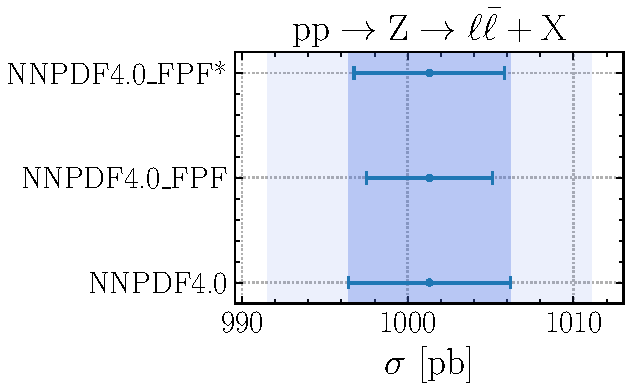
\includegraphics[width=0.32\textwidth]{plots/LHCpheno/NNPDF_DY_14TEV_40_PHENO-integrated.pdf}
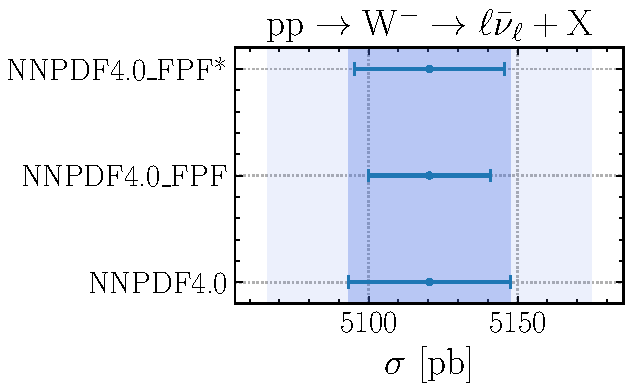
\includegraphics[width=0.32\textwidth]{plots/LHCpheno/NNPDF_WM_14TEV_40_PHENO-integrated.pdf}
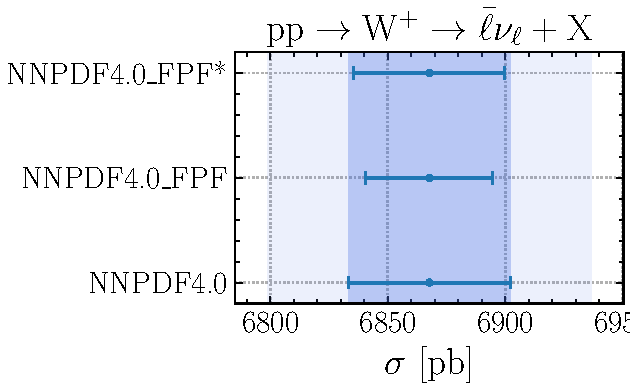
\includegraphics[width=0.32\textwidth]{plots/LHCpheno/NNPDF_WP_14TEV_40_PHENO-integrated.pdf}
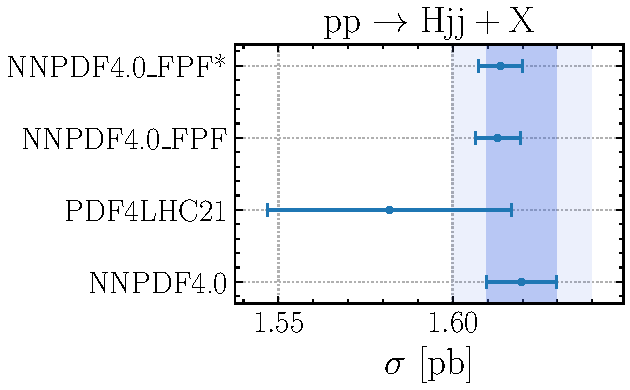
\includegraphics[width=0.32\textwidth]{plots/LHCpheno/NNPDF_HVBF_14TEV_40_PHENO-integrated.pdf}
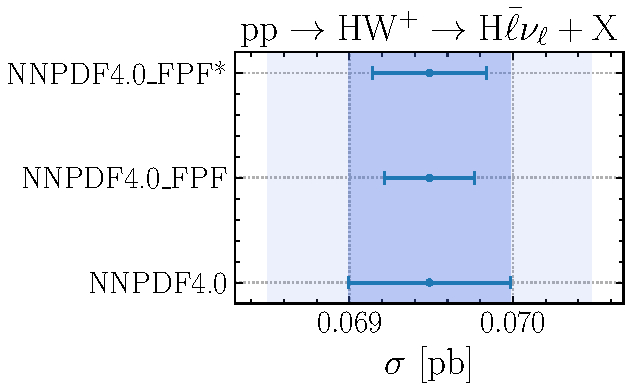
\includegraphics[width=0.32\textwidth]{plots/LHCpheno/NNPDF_HWP_14TEV_40_PHENO-integrated.pdf}
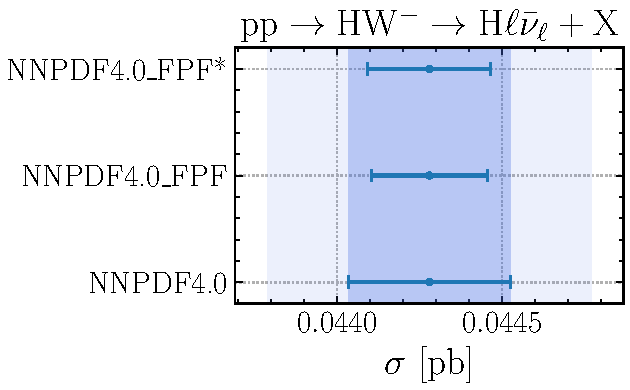
\includegraphics[width=0.32\textwidth]{plots/LHCpheno/NNPDF_HWM_14TEV_40_PHENO-integrated.pdf}
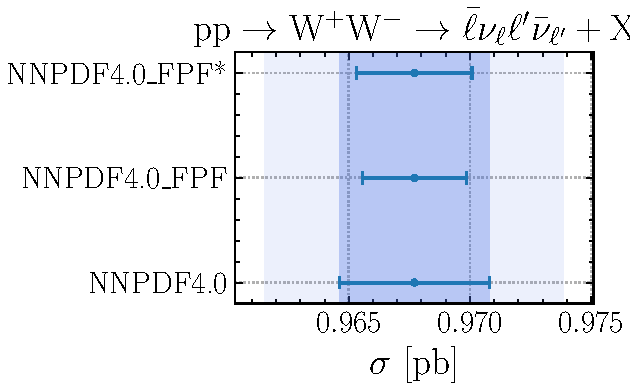
\includegraphics[width=0.32\textwidth]{plots/LHCpheno/NNPDF_WPWM_14TEV_40_PHENO-integrated.pdf}
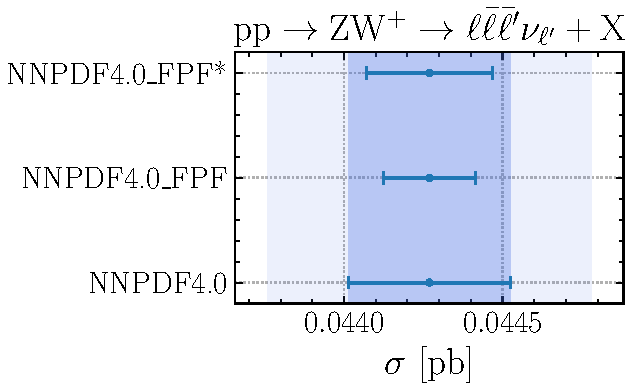
\includegraphics[width=0.32\textwidth]{plots/LHCpheno/NNPDF_WPZ_14TEV_40_PHENO-integrated.pdf}
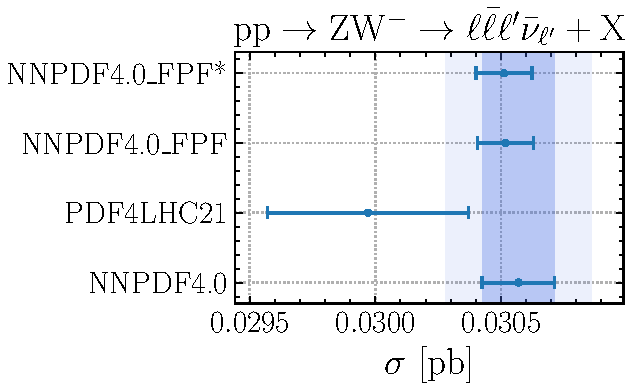
\includegraphics[width=0.32\textwidth]{plots/LHCpheno/NNPDF_WMZ_14TEV_40_PHENO-integrated.pdf}
\caption{Fiducial cross-sections for representative LHC processes at $\sqrt{s}=14$ TeV
evaluated with NNPDF4.0 NNLO, compared with the fits including the FPF structure function projections.
%
For the NNPDF4.0 baseline
prediction, the dark (light) bands indicate the 68\% (95\%) CL uncertainties.
%
The fit labelled as ``\_FPF'' is the one  based on statistical uncertainties,
while that labelled as ``\_FPF$^*$'' also includes systematic errors.
%
The central values are set to be the same as in the original NNPDF4.0 calculation in all cases.
%
See~\cite{NNPDF:2021njg,PDF4LHCWorkingGroup:2022cjn} for the calculational settings.
%
From top to bottom, we show inclusive Drell-Yan production ($Z, W^+, W^-$), Higgs production
in vector-boson fusion, Higgs associated
production, and diboson production ($W^+W^-$, $W^+Z$, $W^-Z$).
%
}
\label{fig:NNPDF40_pheno_integrated}
\end{figure}
%%%%%%%%%%%%%%%%%%%%%%%%%%%%%%%%%%%%%%%%%%%%%%%%%%%%%%%%%%%%%%%%%%%%%%%%


%%%%%%%%%%%%%%%%%%%%%%%%%%%%%%%%%%%%%%%%%%%%%%%%%%%%%%%%%%%%%%%%%%%%%%%%
\begin{figure}[t]
\centering
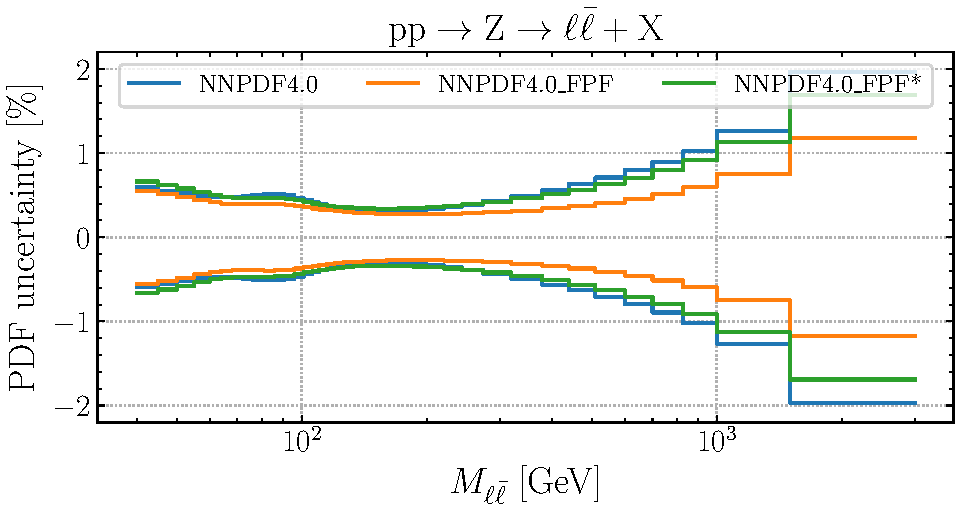
\includegraphics[width=0.49\textwidth]{plots/LHCpheno/NNPDF_DY_14TEV_40_PHENO-global.pdf}
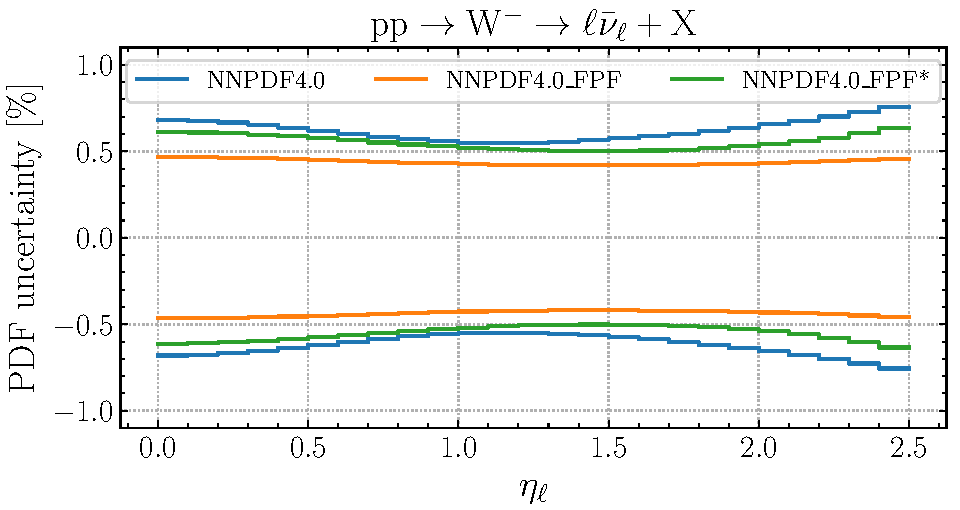
\includegraphics[width=0.49\textwidth]{plots/LHCpheno/NNPDF_WM_14TEV_40_PHENO-global.pdf}
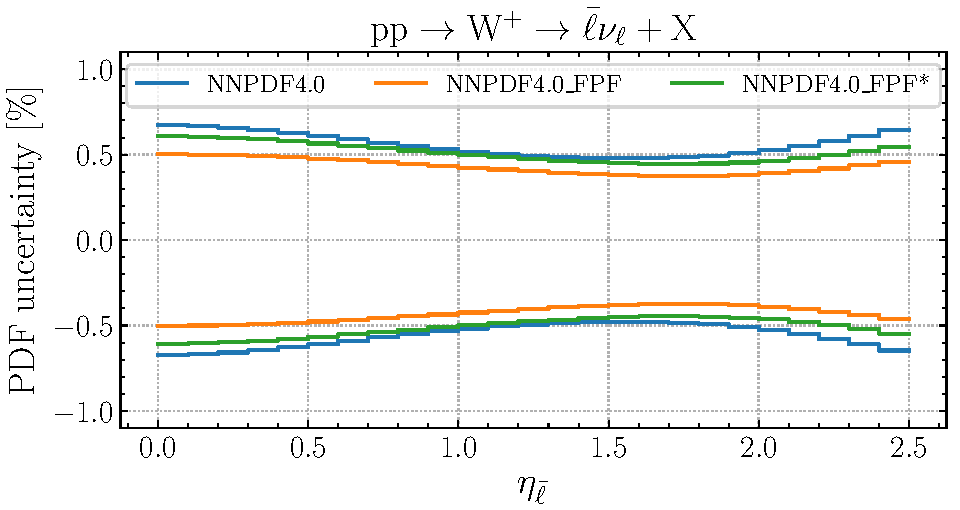
\includegraphics[width=0.49\textwidth]{plots/LHCpheno/NNPDF_WP_14TEV_40_PHENO-global.pdf}
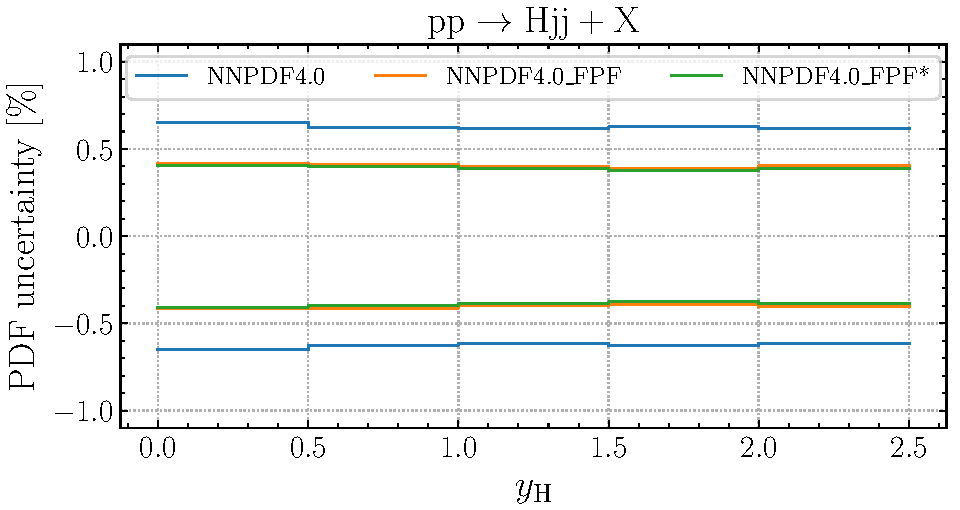
\includegraphics[width=0.49\textwidth]{plots/LHCpheno/NNPDF_HVBF_14TEV_40_PHENO-global.pdf}
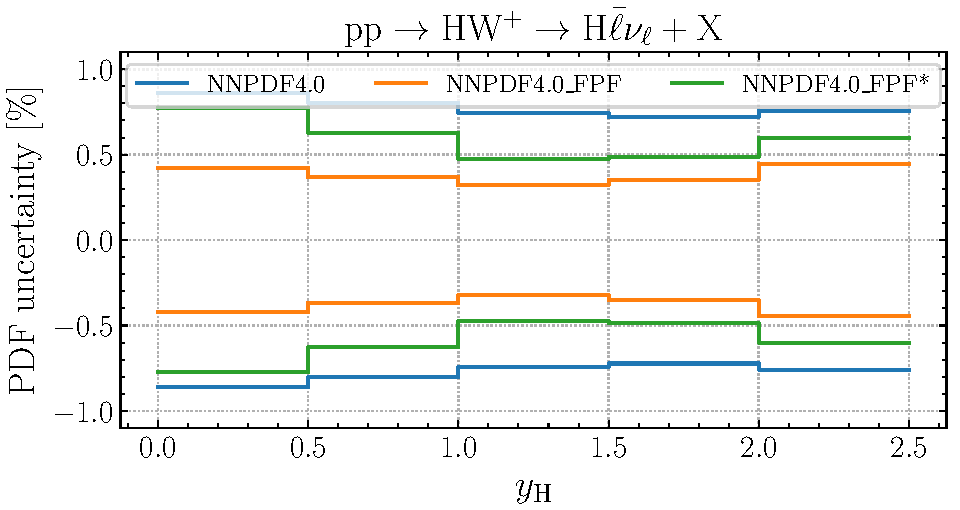
\includegraphics[width=0.49\textwidth]{plots/LHCpheno/NNPDF_HWP_14TEV_40_PHENO-global.pdf}
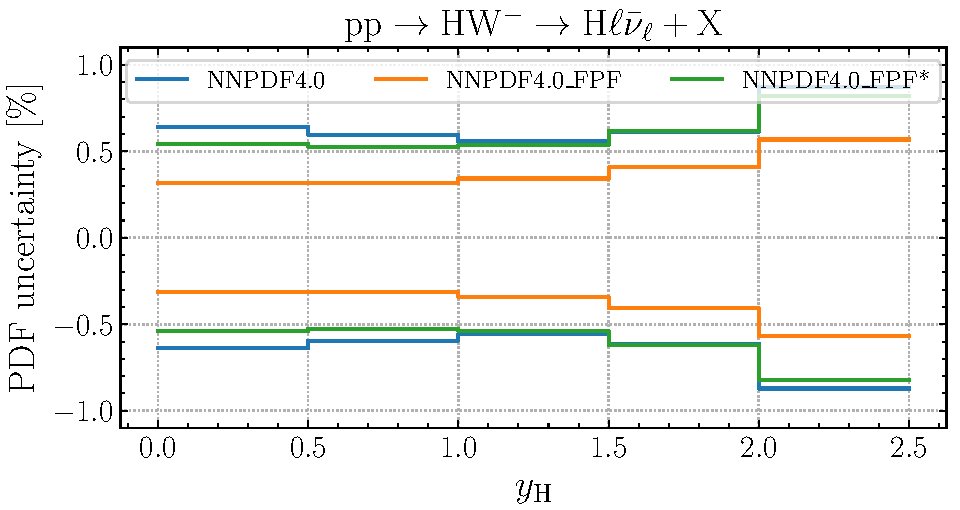
\includegraphics[width=0.49\textwidth]{plots/LHCpheno/NNPDF_HWM_14TEV_40_PHENO-global.pdf}
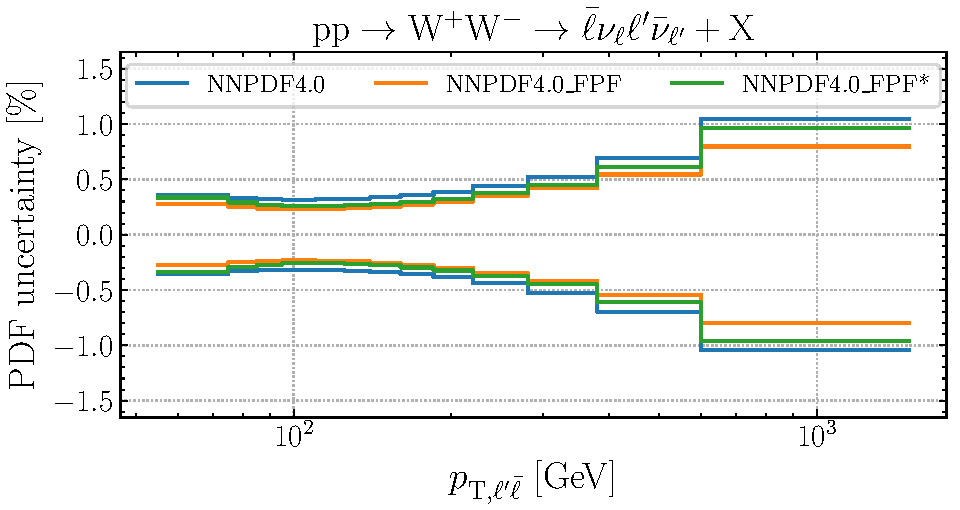
\includegraphics[width=0.49\textwidth]{plots/LHCpheno/NNPDF_WPWM_14TEV_40_PHENO-global.pdf}
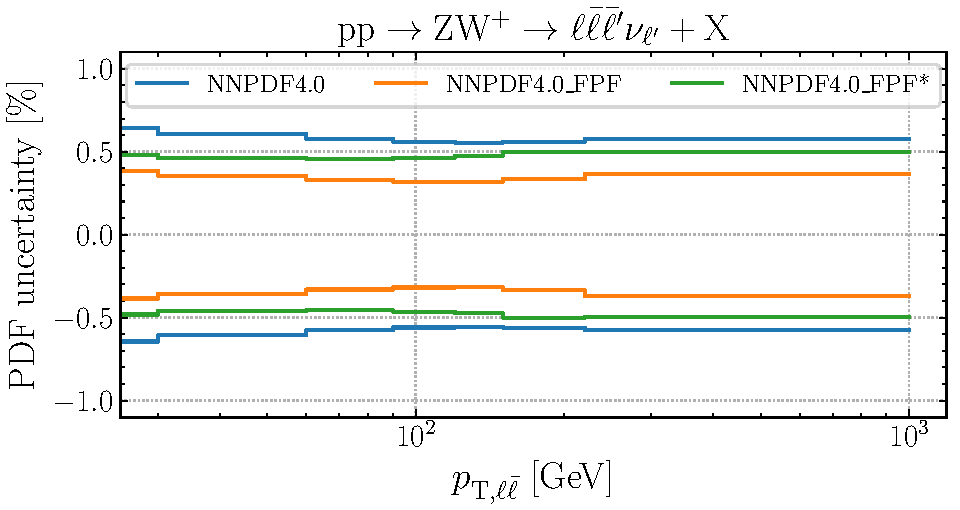
\includegraphics[width=0.49\textwidth]{plots/LHCpheno/NNPDF_WPZ_14TEV_40_PHENO-global.pdf}
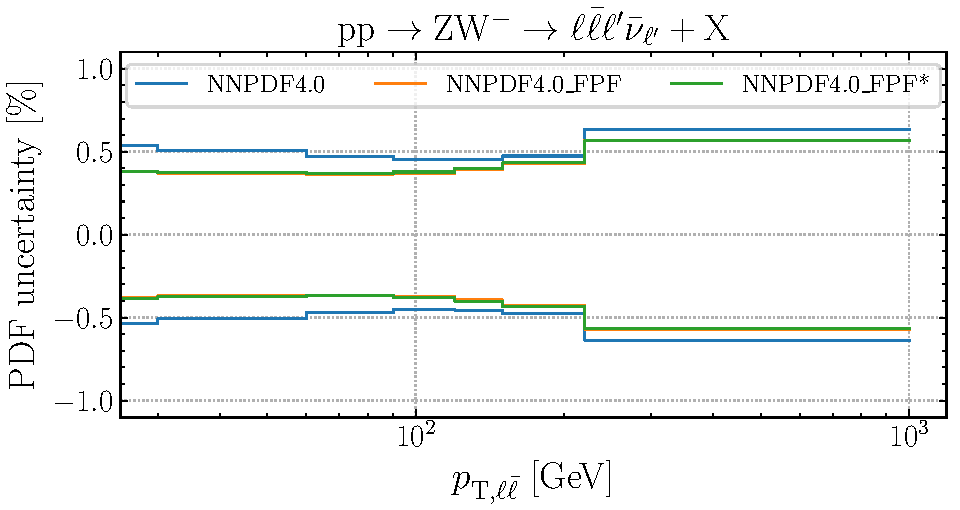
\includegraphics[width=0.49\textwidth]{plots/LHCpheno/NNPDF_WMZ_14TEV_40_PHENO-global.pdf}
\caption{Same as Fig.~\ref{fig:NNPDF40_pheno_integrated}
for the corresponding differential distributions.
%
}
\label{fig:NNPDF40_pheno_differential}
\end{figure}
%%%%%%%%%%%%%%%%%%%%%%%%%%%%%%%%%%%%%%%%%%%%%%%%%%%%%%%%%%%%%%%%%%%%%%%%

Inspection of Figs.~\ref{fig:NNPDF40_pheno_integrated} and~\ref{fig:NNPDF40_pheno_differential}
quantifies the potential of neutrino structure function measurements at the LHC
to improve theoretical predictions for electroweak and high-scale processes at the HL-LHC.
%
Concerning first the fiducial integrated cross-sections, a reduction of PDF
uncertainties is observed for all processes,
including for $W^+$ production relevant for $m_W$ measurements, and its specific  magnitude depends
on the underlying scattering reaction.
%
This finding also applies for Higgs associated production with vector bosons and in vector-boson-scattering,
with for example
PDF uncertainties in $hW^+$ reduced by up to a factor two thanks to the FPF measurements.
%
Similar remarks apply to the diboson cross-sections, with in this case the largest
improvement observed for $ZW^+$ channel.
%
Reassuringly, LHC predictions based on the fits with FPF pseudo-data are stable
upon the inclusion of the experimental systematic uncertainties in the fit.

In the case of the differential cross-sections shown in Fig.~\ref{fig:NNPDF40_pheno_differential},
we observe how the impact of the FPF structure functions on LHC observables depends
on the hard-scattering scale.
%
For instance, searches for heavy-resonances in the high-mass tail of the Drell-Yan
distributions are going to be improved by FPF data.
%
The same applies for diboson prediction, and in the case of the $ZW^+$ channel we observe
an improvement spatially in the low $p_{T,\ell\bar{\ell}}$ region.
%
For the Higgs production processes, the PDF uncertainty in the theory predictions is relatively
stable as a function of the rapidity.
%
The effects of accounting for systematic uncertainties in the fit are somewhat more visible
here as compared to the inclusive cross-sections, indicating that they affect mostly
the tails, rather than the bulk, of the distributions, and in particular the large-$x$
behaviour of the PDFs.

The studies presented in this section provide only a first glimpse of the potential
of neutrino DIS measurements at the LHC to inform predictions for high-$p_T$ processes.


